%
% Estructura de pruebas.
% Análisis y diseño de programa tokenizador, reporte técnico.
%
% Proyecto Lovelace.
%

\paragraph{Estructura de pruebas de unidades}

A la par que se implementa el programa descrito hasta ahora, se crearán
\glspl{gl:prueba_de_unidad} y \glspl{gl:prueba_de_componente}. La idea de
combinar el desarrollo de pruebas con el proceso de implementación es encontrar
problemas en una etapa temprana, facilitar el cambio de código existente y
simplificar la integración de nuevos componentes. La ejecución de las pruebas
está ligada a un proceso de integración continua, de forma que con
cada pequeño cambio (con cada \textit{commit}) se ejecute desde cero todo el
proceso de compilación y pruebas.

Algunos lenguajes (como Python) cuentan con un modelo de pruebas integrado;
otros (como Java o Javascript) cuentan con librerías muy populares (JUnit o
Karma). En el caso de C++ no hay ningún soporte desde el propio lenguaje, y
entre las librerías existentes tampoco hay ninguna que se haya establecido como
favorita. Es por eso que se decidió crear una estructura de pruebas propia:
en la figura \ref{clases_pruebas} se muestra la estructura de las clases de
pruebas para todo el programa. Este muestra a modo de ejemplo solamente algunas
de las clases; todas las demás siguen el mismo esquema.

Las tres clases de la derecha, dentro del paquete de utilidades, son para
agrupar y gestionar de una forma genérica a todas las pruebas. Un conjunto de
pruebas tiene un lista de la clase Prueba. La clase Prueba tiene una lista de
funciones de prueba. Las funciones de prueba tienen una descripción y un
apuntador a una función (la propia prueba). Todas las pruebas dentro del
programa deben ser especificaciones de la clase prueba. El estándar es que una
clase de prueba defina todas las funciones (booleanas y estáticas) que necesite
y las agregue a la lista de pruebas de la superclase.

Existen dos paquetes para agrupar a las pruebas: uno para lo que hay en
implementaciones y otro para las utilidades. Lo ideal es que por cada parte del
código en donde haya lógica no trivial se hagan funciones de prueba. Así, si hay
una clase \textit{Ejemplo}, debe de existir una clase \textit{EjemploPrueba}
que capture el comportamiento esperado de \textit{Ejemplo}. En algunos casos,
las clases de prueba deben tener acceso a lo que la propia clase encapsula
(miembros privados o protegidos), por lo que la clase de prueba debe ser amiga
de la clase probada.

\begin{figure}
  \begin{center}
    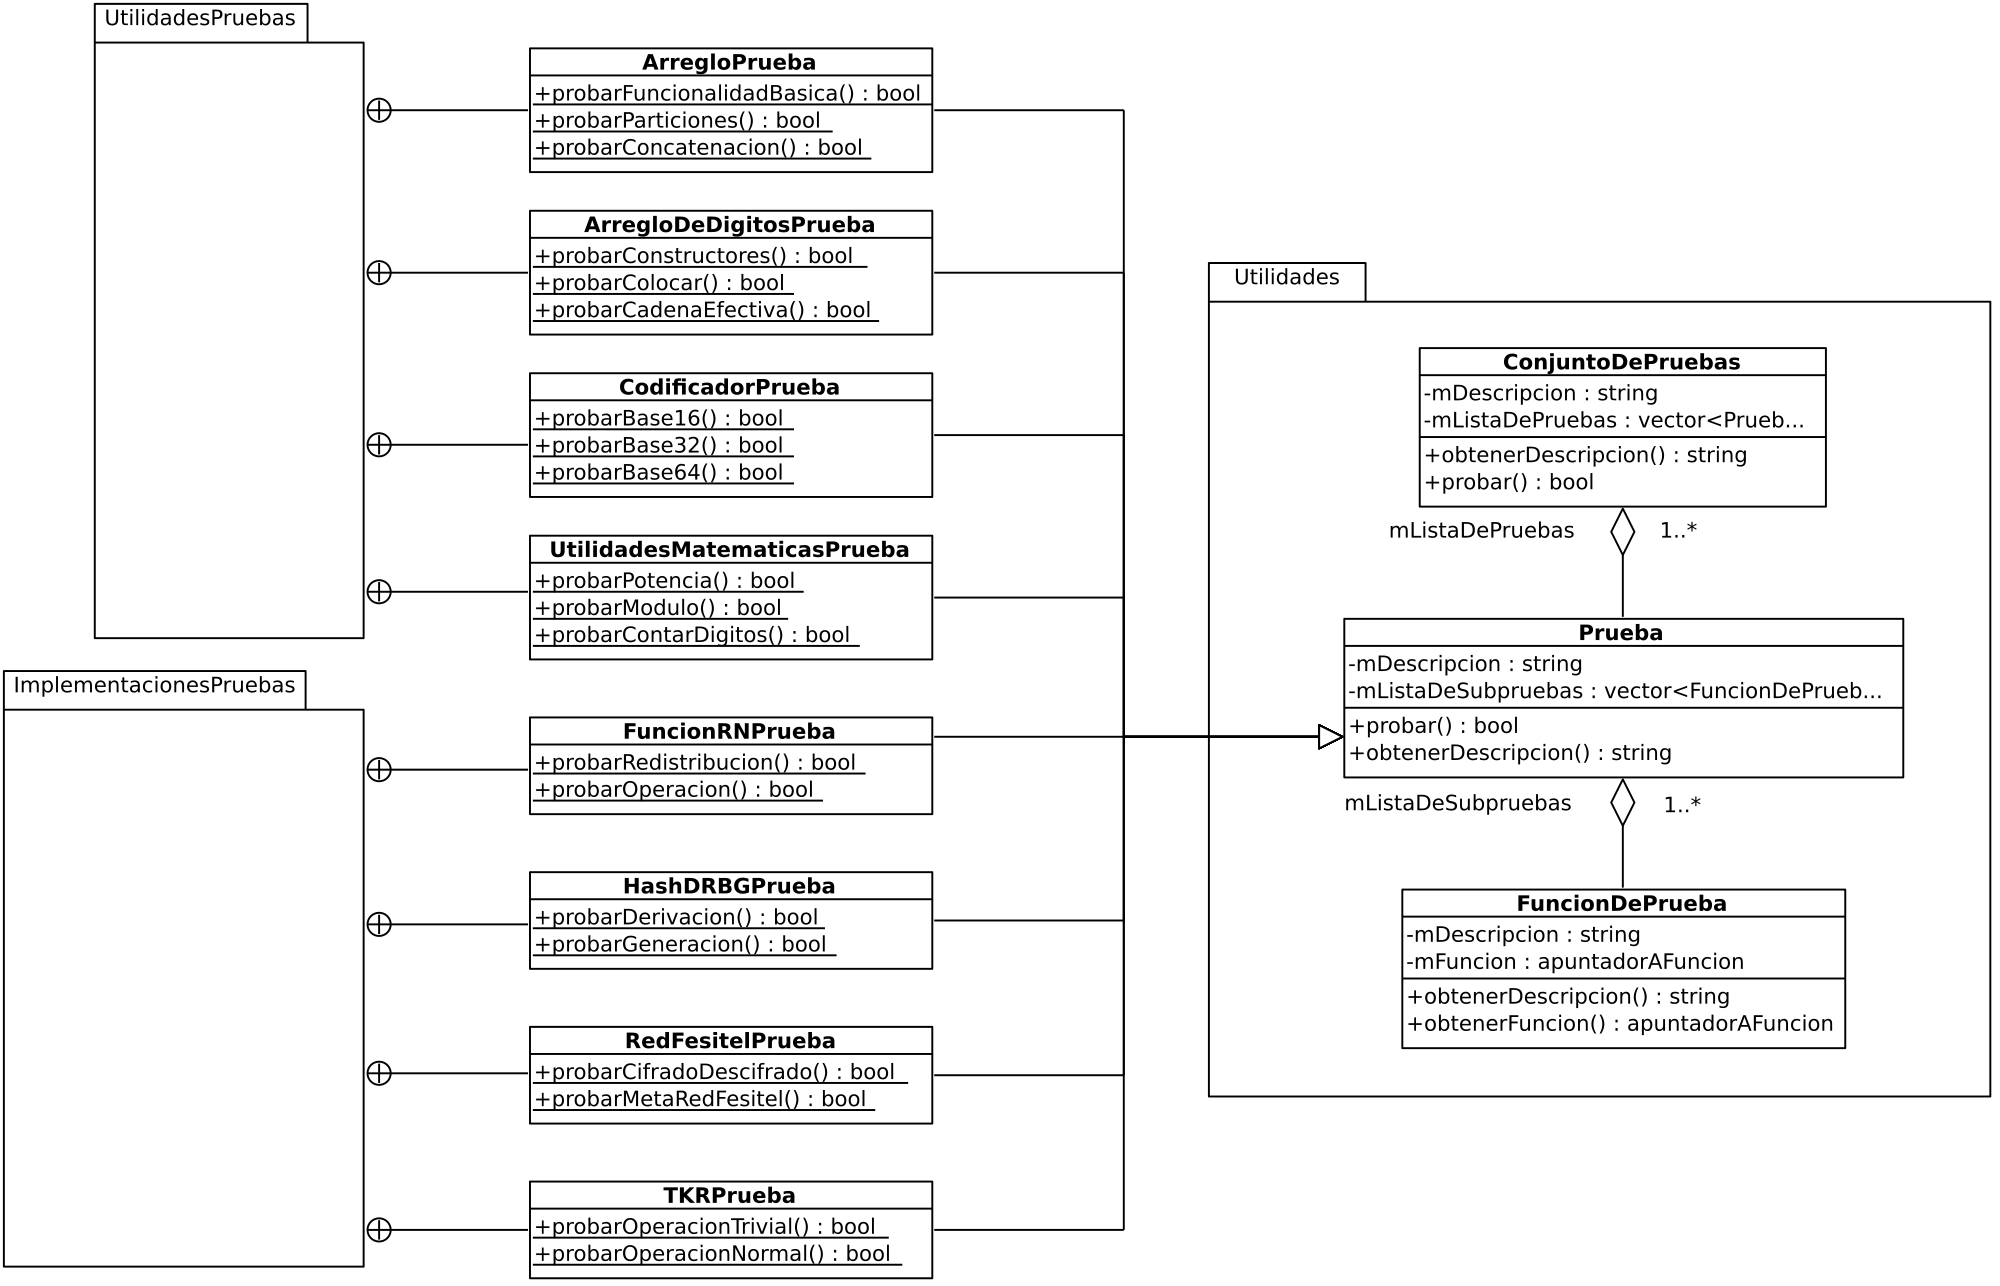
\includegraphics[width=1.0\linewidth]{diagramas/pruebas.png}
    \caption{Diagrama de clases de la estructura de pruebas.}
    \label{clases_pruebas}
  \end{center}
\end{figure}
